%
\chapter{2D Simulation of Capacitively Coupled RF Discharges}\label{sec:chapter_twodccrf}
%
    After using a 1d3v PIC algorithm to investigate and understand the dynamics of negative oxygen ions in an axial approximation of a symmetrical radio frequency plasma, we will now look at the influence of asymmetry effects in capacitively coupled discharges. Therefore, a 2d3v PIC-MCC simulation is used, where the axial and radial direction is resolved. In this chapter we want to investigate the impact of self-bias and different asymmetry conditions on the development of a plasma, e.g. by varying the area ratios of electrodes and the self-bias voltage. The dynamics and energy distribution of negative ions are discussed in more detail.
%
    \section{Simulated Discharge}\label{sec:simulatedd_dis}
%	
        The cylindrical setup in~\cite{Scheuer15} is represented by a 2d3v PIC simulation with two spatial dimensions $(r,z)$ and the full velocity triplet $\vec{v}=(v\ix{r},v_{\vartheta},v\ix{z})$. They form a two-dimensional mesh of grid points in radial and axial direction. Figure~\ref{fig:radialcylinder} shows the full cylinder on top of the simulation domain. The cylindrical metrics has to be taken into account for fluxes and densities. A weighting methody proposed by Verboncoeur et al.~\cite{Verboncoeur01} is used.\\
	    Because the radial dimension has been introduced, additional transport occurs in this direction. This additional radial loss of particles compared with the 1D situation requires higher production rates to sustain a stable discharge.
%	    
	    \clearpage
        \begin{figure}[!t]
            \centering
            \begin{subfigure}{0.49\textwidth}
                \centering
				\includegraphics[height=0.17\textheight]%
					{figures/radial_cylinder.png}
                \caption{Simulation domain.}
            \end{subfigure}
            \begin{subfigure}{0.49\textwidth}
                \centering
				\includegraphics[height=0.17\textheight]%
					{figures/domain_slice.png}
                \caption{Plasma bulk and boundary conditions.}
            \end{subfigure}
            \caption[Schematic of the simulation domain]{%
			    Cylindrical schematic of the simulated %
			    discharge.~\cite{Matthias15}}%
			\label{fig:radialcylinder}
      \end{figure}
%        
		In order to realise an asymmetric discharge the area ratio of driven and grounded electrodes are varied. The large area of the grounded vessel walls have to be considered as well. For the self-bias voltage and negative surface ionisation efficiency experimental values from~\cite{Meichsner13,Kullig12} are used.
%
		\par\bigskip
		To assure the validity of this algorithm, we will compare the results of the one-dimensional model with those of the 2d3v simulation. We consider this as sufficient, because the 1D PIC approach is a well-established method and has been widely approved~\cite{Matyash07oxIII,Bronold07b,Matthias15}. Subsequently, the influence of different asymmetries, e.g. sizes of driven and grounded electrodes, self bias voltage and secondary ion emission from surfaces on the discharge, will be investigated.
%
    \section[Validation of Simulation Method by Comparison with 1d3v PIC]%
    {Validation of Simulation Method by \\
    Comparison with 1d3v PIC - The symmetric discharge}\label{sec:validationtwod}
%    
        The possible solutions in a two-dimensional simulation model are more complex than those of the 1D counterpart. The additional radial transport leads to modifications of the 1D solution and the system is much more sensitive to boundary conditions.
        A 1D PIC simulation is always intrinsically symmetric, whereas in 2D one has to take care to ensure this. In fact, the possibility for asymmetric solutions is motivating the use of 2D, because this is needed to get more realistic conditions than a 1D code. To highlight this, discharges with different boundary conditions and driver configurations are simulated later on, which then will be compared to the results from the one-dimensional model.\\
%
        \clearpage
        \begin{figure}[!t]
            \centering
            \includegraphics[height=0.4\textheight]%
                {figures/results/2D/45431/onedtwod_45431_denscompare.png}
            \caption[Comparison of 1D and 2D axial density profiles]{%
                Comparison between 1D and 2D results %
                of densities at the axis of a cylindrical discharge at %
                \SI{5}{\pascal} and \SI{400}{\volt}}
            \label{fig:twodonedcompare}
        \end{figure}
        \vfill
        \begin{figure}[!h]
            \centering
            \includegraphics[height=0.4\textheight]%
                {figures/results/2D/45431/onedtwod_45431_phicompare.png}
            \caption[Comparison between 1D and 2D axial potential profile]{%
                Comparison between 1D and 2D results %
                of plasma potential at the axis of a cylindrical %
                discharge at \SI{5}{\pascal} and \SI{400}{\volt}}
            \label{fig:twodonedcomparepot}
        \end{figure}
        \clearpage
%       
        The 1D code is used to simulate the central part of a discharge with a length of  \SI{6.72}{\centi\metre} at \SI{5}{\pascal} and a driver voltage of \SI{400}{\volt}. Again, negative surface ions are produced at the cathode. The driven electrode is on the right hand side at $z=\,$\SI{6.72}{\centi\metre}, whereas the anode at $z=0$ is grounded. The electrodes are mirror-inverted to the 2D case.\\
        First, a fully symmetrical discharge is simulated in 2D. The use of one grounded and one driven electrode does not yield the correct result, which will be discussed later. Instead, one applies an external excitation of \SI{400}{\volt} on both electrodes, at $z=0$ and $z=574\lambda\ix{Db}/2$, respectively, with a difference in phase of $\pi$. No self-bias will be introduced. The electrode sizes were chosen to be equal with \SI{2.25}{\centi\meter} at one quarter of the domains radius, which itself was set to \SI{8.98}{\centi\meter}. This corresponds to 175. The electrodes are driven sinusoidally at \SI{13.56e6}{\hertz} with \SI{400}{V} peak voltage. The boundary conditions above the electrodes at the left and right domain boundaries are zero electric field $\vec{E}=0$. The outer radial boundary is set to ground representing the vessel wall.\\
        A comparison of density profiles and potential is given in~\autoref{fig:twodonedcompare} and~\autoref{fig:twodonedcomparepot}. The dotted lines show results from the 2D, and solid ones from the 1D simulation. The density and potential profiles in 2D are averaged over a few cells in radial direction, e.g., 20 -- 30 cells to reduce the statistical errors.\\
        The bulk densities are in good agreement within their statistical errors in the centre of the discharge, e.g\@ approximately\SIrange{1.8}{5.2}{\centi\metre}. The 2D density profiles have the same features as the 1D ones: the charged species form a well-defined plasma bulk around the centre of the discharge, in which the sum of electron and negative ion density equals the ion density of positive ions.\\
        Differences occur towards the plasma sheaths. The space charge areas for the 2D case are larger in front of both electrodes, approximately 60$\,\lambda\ix{Db}/2$. Conclusively, the densities decay much faster from the bulk. This is due to the additional influence of the continuity condition for electron and ion flux by the plasma boundaries and electrode edges. They have a great influence on the density and potential, as it was described by~\autoref{equ:ionandelectrondens}. There are additional radial transport processes, which occur in the 2D simulation. They lead to a loss of particles, which is equivalent to an outwards flux. In areas where the confinement in the bulk is no longer given, particles can escape from the plasma.\\
        In \autoref{fig:twodonedcomparefull} the densities and potential for the full 2D domain is shown. The plasma bulk is shaped self-consistently by the influence of the 2D boundaries. In the logarithmic plot of the electron density the small areas around the whole plasma show up clearly where the density drops rapidly.\\
%        
        \begin{figure}[!t]
            \centering
            \includegraphics[width=1.0\textwidth]%
                {figures/results/2D/45431/twod_alldensphi_45431.png}
            \caption[2D particle densities and potential]{%
                Spatially 2D particle densities %
                on a logarithmic scale. Potential %
                of a simulated discharge at \SI{5}{Pa} and %
                \SI{400}{\volt}. The top boundary of the domain %
                is grounded, both electrodes are driven %
                and the remaining parts are allowed to float.}
            \label{fig:twodonedcomparefull}
        \end{figure}
 %       
        Regions with differences of electron, negative and positive ion density are limited to the plasma sheath: electrons, and eventually the likewise negatively charged ions are depleted in the space charge sheath in front of the electrodes. The positive ions however are accelerated and therefore have a higher density here.\\
        The same surface electron attachment process as described in~\autoref{sec:surfaceeffects} for the 1D simulation is implemented at the left driven electrode. Neutrals hitting the wall can attain an additional electron and are charged negatively. These negatively charged ions are then accelerated within the sheath towards the bulk. They undergo electron detachment within the sheath, so that the electron density in front of the left electrode is increased.\\
        In this symmetric simulation only the left electrode has this surface ionisation process in order to elucidate the influence of this process on the plasma. For the asymmetric case only the left electrode will be driven and consequently the only one with electron attachment.
        The plasma potential in~\autoref{fig:twodonedcomparepot} is an average over a few cells from the results shown in~\autoref{fig:twodonedcomparefull}. Again, the results from 1D and 2D agree very well. The mean plasma potential is found to be approximately \SI{290}{V} across the plasma bulk between \SIrange{1.5}{5.5}{\centi\metre}. However, the voltage drop towards both electrodes is found to be steeper for 2D, which is the consequence of the influence from the boundaries of the plasma and electrode edges.\\
        The potential of the 2D simulation in~\autoref{fig:twodonedcomparefull} very well highlights the findings from before. The mean plasma potential is constant across the bulk. The average potential of the electrodes rest at \SI{0}{\volt}, while the grounded part of the vessel on top confines the plasma in the radial direction. The remaining parts of the domain above the electrodes are allowed to float, e.g\@ follow the plasma potential, which implies $\vec{E}=0$. 
%
        \par%
        In summary, if boundary conditions and symmetry are adjusted accordingly, the 2D code matches the 1D code very well. Therefore the used 2D PIC code can now be used to investigate the influence of asymmetry effects and their impact on the plasma dynamic, not possible in the 1D model. The next section is devoted to the discussion of different boundary conditions with respect to the symmetrical 1D case.
%        
    \section{Influence of Asymmetric Boundary Conditions in 2D}
%        
        In the following the impact of different combinations of boundary conditions on the development of a low-pressure ccrf plasma is considered. Firstly the same discharge is modelled like in 1D, where one electrode is driven and one is grounded, producing now asymmetry effects. The left electrode is driven sinusoidally with a voltage of \SI{400}{\volt} at \SI{13.56e6}{\hertz}. Surface processes of negative ions are considered on the cathode. Again, no self bias is applied.\\
        The axial potential profile shows a similar behaviour as the 1D calculations, see Figure~\ref{fig:twodonedcomparefalsepot}. Differences in the width of the sheath are observed. The corresponding potential drop in the plasma sheath between 0 -- \SI{1}{\centi\metre} and 5 -- \SI{6.7}{\centi\metre} respectively is also different. In front of the cathode the drop is much steeper than at the anode. Conclusively the sheath is much smaller on that side.\\
        Asymmetries introduced by the different driver configuration are pronounced in the resulting density profiles of the charged plasma species seen in Figure~\ref{fig:twodonedcomparefalse}. Densities are shifted towards the driven electrode at \SI{0}{\centi\metre}. 
%
        \clearpage
        \begin{figure}
            \centering
            \includegraphics[width=0.9\textwidth]%
                {figures/results/2D/43748/45365prs_pot.png}
            \caption[Axial profil of plama potential from 2D]{%
                Axial profile of plasma potential from 2D %
                simulation at \SI{400}{\volt}. Only the left hand %
                electrode at $z=0$ was driven. It resembles 1D results.}
            \label{fig:twodonedcomparefalsepot}
        \end{figure}
        \vfill
        \begin{figure}[!t] %% THIS IS ASYMMETRIC
            \centering
            \includegraphics[width=0.9\textwidth]%
                {figures/results/2D/43748/45365_dens.png}
            \caption[Axial profile of 2D densities]{%
                Axial profile of densities of the 2D %
                simulation of a discharge at %
                \SI{5}{\pascal} and \SI{400}{\volt}. Only the left hand %
                electrode at $z=0$ was driven, while the other was grounded.}
            \label{fig:twodonedcomparefalse}
        \end{figure}
        \clearpage
%        
        One can easily see the large difference between the ion density in front of the two electrodes. At the cathode $n\ix{i}$ is between 3 -- 4 times higher than at the anode.\\
        This is a consequence of the global asymmetry between the areas of driven and grounded walls. The area of anode and upper wall is much bigger than the area of the driven electrode.  Since those are in imbalance, the particle fluxes on the driven electrode need to be higher. The change in the sheath in front of the anode is generated. Therefore different potential drops establish which is shown in ~\autoref{fig:twodonedcomparefalsepot}. One can see there that also the mean and phase-resolved plasma potential is shifted as a consequence of asymmetry.
%        
        \par\bigskip%
        By the results of this simulation, where the same boundary conditions like in 1D have been applied, we have seen that an asymmetrical setup yields strong deviations from the earlier results. Plasma potential and densities change according to the global flux condition on grounded and driven walls. Like it was discussed in~\autoref{sec:sheathphysics}, in a laboratory ccrf discharge asymmetries lead to the development of a self bias voltage. Thus we introduce this property to the 2D simulation. Values are chosen between \SIrange{-200}{-500}{\volt} from experimental results in~\cite{Kullig12,Meichsner13} and added as a dc-offset to the potential of the driven cathode.
%
        \par\bigskip
        Firstly I will simulate two different asymmetric discharge configurations. The results of potential, ion density and axial ion velocity $v\ix{z}$ is shown in~\autoref{fig:asym_comparebig}. This is only a small selection of the full diagnostics set. A comparison between the axial energy distribution function for all species in those discharges and the remaining densities can be found in~\autoref{fig:app_dens} through~\autoref{fig:app_edf_ni}. Both discharges were \SI{8.98}{\centi\metre} in diameter and had an electrode gap of \SI{6.72}{\centi\metre}. At a Debye length of \SI{0.0235}{\centi\metre} this resulted in a domain size of $(764\times572)\cdot\lambda\ix{Db}/2$ in both directions respectively. They were equally driven at a voltage of \SI{400}{\volt} and rf frequency of \SI{13.56e6}{\hertz}.\\
        The discharge on the left side of the plot panel was driven at the bottom quarter of the left domain boundary, e.g\@ between 0 and \SI{22.7}{\centi\metre}, with an additional \SI{-500}{\volt} self bias. Because the rest of the boundaries were set to ground a large asymmetry sustained, which conclusively resulted in a high dc offset. The one on the right side was powered on both electrodes up to the same height. The left and top part of the boundary where grounded, while the right was allowed to float.\\
        The first two figures in one column show the potential and ion density. The left has an average plasma potential of around \SI{300}{\volt} across the bulk. On the cathode however this is equal to the self bias offset. Between \SIrange{0.5}{5.7}{\centi\metre} and up to \SI{5}{\centi\metre} the bulk core extends. Plasma potential and ion density are shifted towards the cathode. Sheaths in front of both electrodes are also asymmetric. Before the cathode the ion density is higher by at least one order of magnitude, while the space charge is roughly half the size of the opposing sheath. Density and potential drop at the left electrode are obviously quite large, which means that ions are accelerated at this point to match the current onto other compartments of the grounded vessel. Because of the very large ratio between grounded and driven walls, the cathode sheath yields a much stronger ion current pointing outwards, which can be seen the bottom plot of the axial ion velocity. Here one can see that the acceleration is larger and the ions quickly reach the Bohm velocity of around \SI{1.15e6}{\meter\per\second}, while this process extends over a greater distance in front of the grounded anode.\\
        The figures on the right side however yield another picture. The plasma core is shifted and bend towards the floating boundary above the right hand side electrode. The bulk establishes between \SIrange{2}{5}{\centi\metre}, while the height it makes contact with the wall is around \SI{4}{\centi\metre}. The overall density of the ion particles in this discharge is around one order of magnitude smaller.\\
        Potential drops on both sides are again steep, but not as much as for the comparing setup. Also the average plasma potential is found to be between \SIrange{800}{1000}{\volt}, which is much higher than the results from before. On the cathode the mean value is again the self bias voltage. The plasma sheaths are around \SI{2}{\centi\metre} in thickness in front of both electrodes. Corresponding ion densities are equal in between the cathode and anode. However, towards the edge of the bulk near the floating wall the density increases again. Besides the shape of the plasma core, the smaller asymmetry in this simulation led to a smaller sheath and overall density, as well as velocities which can be seen on the bottom of the panel. The acceleration of positive ions takes longer and the currents onto both electrodes are lower in comparison to the left discharge.
%
        \clearpage
        \begin{figure}[!h]
            \centering
            \begin{subfigure}{0.49\textwidth}
                \includegraphics[height=0.3\textheight]%
                    {figures/results/2D/44332/phi.png}
            \end{subfigure}
            \begin{subfigure}{0.49\textwidth}
                \includegraphics[height=0.3\textheight]%
                    {figures/results/2D/44426/phi.png}
            \end{subfigure}
            \newline
            %\caption[]{%
            %    }
            %\label{fig:}
        %\end{figure}
        %\begin{figure}
            %\centering
            \begin{subfigure}{0.49\textwidth}
                \includegraphics[height=0.3\textheight]%
                    {figures/results/2D/44332/i_dens.png}
            \end{subfigure}
            \begin{subfigure}{0.49\textwidth}
                \includegraphics[height=0.3\textheight]%
                    {figures/results/2D/44426/i_dens.png}
            \end{subfigure}
            \newline
            %\caption[]{%
            %    }
            %\label{fig:}
        %\end{figure}
        %\begin{figure}
            %\centering
            \begin{subfigure}{0.49\textwidth}
                \includegraphics[height=0.3\textheight]%
                    {figures/results/2D/44332/i_velz.png}
            \end{subfigure}
            \begin{subfigure}{0.49\textwidth}
                \includegraphics[height=0.3\textheight]%
                    {figures/results/2D/44426/i_velz.png}
            \end{subfigure}
            \caption[Comparison between asymmetrically driven discharges]{%
                Comparison of potential (\textbf{top}), ion density (\textbf{mid}) and %
                axial ion velocity (\textbf{bottom}) for two differently configured discharges. %
                The \textbf{left} is driven on the left side and a grounded box is put around it.
                On the \textbf{right} both electrodes are driven, but the top left part is %
                set to ground and the right above the anode is allowed to float. Self bias voltages %
                were \SI{-500}{\volt} and \SI{-400}{\volt} respectively.}
            \label{fig:asym_comparebig}
        \end{figure}
        \clearpage
%
    \clearpage
    \section{Self Bias and Negative Ion Dynamics}
%    
        We will now study the dynamics of negative ions in a 2D simulation of rf discharges with a self bias voltage on the driven electrode. The results of this section stand in comparison to the findings from~\autoref{sec:chapter_onedcomparison}, while the introduced self bias is expected to have an important impact on the EDF of negative ions.\\
        The simulation dimensions have been changed slightly. A cathode with a radius of \SI{1.5}{\centi\metre} and an anode with a radius of \SI{4.5}{\centi\metre} is used in the model and a all other boundary conditions are set to ground potential grounded. The electrode gap is about \SI{2.5}{\centi\metre}. We chose an electron temperature of \SI{6}{\electronvolt} and density of \SI{5e9}{\per\cubic\centi\metre} for the dimensionless scaling parameters. This gives a cell width of \SI{0.012}{\centi\metre} and a time step of \SI{5.02e-11}{\second}. The corresponding simulation dimensions were 125 cells for the cathode, 375 cells for the anode and an electrode gap of 208 cells.\\ 
         In figure (\ref{fig:dens_ni}) the number density of negative ions is shown for pressures of \SI{10}{\pascal} and \SI{5}{\pascal} with an applied voltage of \SI{400}{\volt}. One can see that the bulk region is deformed at the cathode side due to the self-bias voltage of \SI{-200}{\volt} leading to a reduced electron flux towards the cathode.\\
        There is a higher flux of ions towards the cathode than to the anode due to the self-bias voltage. In the 1D simulation the total ion flux towards the cathode and the cathode sheath are underestimated, because a self-bias effect can not exist. The density distributions have still the same form, where ions are mostly confined in the bulk around the centre of the discharge and their number increases towards the cathode because of an additional particle current from the wall.\\
        In~\autoref{fig:velz_ni} the axial component $v\ix{z}$ of the particle velocity is shown. One can easily see that the negative ions are nearly stationary in the bulk, while at the sheath edges they follow the external electric field. Here they are accelerated in direction of the opposite electrode. At the cathode however the negative ion velocity is much higher than in the bulk or the sheaths. They are are heavily accelerated by an electric field from the excitation and self bias voltage. For lower pressures the probability of energy loss and charge exchange collisions with neutral gas molecules is lower, which is why~\autoref{fig:velz_ni} at \SI{6}{\pascal} also shows high velocities in front of the anode. Fast surface ions may fly through the bulk because their mean free paths are sufficiently large and impinge on the anode.\\
        To investigate this process we will have a look at the energy distributions of the negative ions. Following the arguments of the one-dimensional model the injected anions should not be able to stay in the discharge, due to the additional energy from the self-bias voltage.
%        
        \clearpage
        \begin{figure}[!t]
            \centering
            \begin{subfigure}{0.49\textwidth}
                \includegraphics[width=1.0\textwidth]%
                    {figures/SFB/ni_dens_25690000.png}
                \caption{\SI{10}{\pascal}.}
            \end{subfigure}
            \begin{subfigure}{0.49\textwidth}
                \includegraphics[width=1.0\textwidth]%
                    {figures/SFB/ni_dens_25830000.png}
                \caption{\SI{6}{\pascal}.}
            \end{subfigure}
            \caption[Negative ion density from 2D at different pressures]{%
                Logarithmic plot of negative ion %
                particle density distribution at different %
                discharge pressures.}
            \label{fig:dens_ni}
        \end{figure}
        \vfill
        \begin{figure}[!b]
            \centering
            \begin{subfigure}{0.49\textwidth}
                \includegraphics[width=1.0\textwidth]%
                    {figures/SFB/velni_z_25690000.png}
                \caption{\SI{10}{\pascal}.}
            \end{subfigure}
            \begin{subfigure}{0.49\textwidth}
                \includegraphics[width=1.0\textwidth]%
                    {figures/SFB/velni_z_25830000.png}
                \caption{\SI{6}{\pascal}.}
            \end{subfigure}
            \caption[Axial velocity of negative ions in 2D at different pressures]{%
                Axial velocity $v\ix{z}$ of negative ions %
                at different discharge pressures.}
            \label{fig:velz_ni}
        \end{figure}
        \clearpage
%       
        \begin{figure}[!b]
            \centering
            \includegraphics[width=0.9\textwidth]%
                {figures/SFB/MORE/ni_distz.png}
            \caption[Axial spatio-temporally resolved EDF of negative ions in 2D]{%
                Spatio-energetically resolved logarithmic %
                plot of negative ion EDF at \SI{6}{\pascal} and %
                $U\ix{rf}=\,$\SI{400}{\volt} and $U\ix{sb}=\,$\SI{-200}{\volt}.}
            \label{fig:twodedf_ni}
        \end{figure}
%        
        In~\autoref{fig:twodedf_ni} the EDF of negative ions is shown. Obviously the distribution is strongly asymmetric. A peak structure located at the cathode can be found, which starts around \SI{0}{\electronvolt} and rises to nearly \SI{200}{\electronvolt} when proceeding further along the axis. At \SI{0.7}{\centi\metre}, which is the approximate sheath thickness taken from~\autoref{fig:dens_ni}, the structure reaches the maximum energy. Though the particle counts decrease towards the anode, a non-negligible amount of negative ions reaches the opposing electrode with high energies, e.g\@ >\SI{150}{\electronvolt}. This is due to the strong acceleration by an electric field from the combined voltage of self bias and external excitation.\\
        Besides this part of the negative ions species, the majority of particles is found to be at low energies between the discharge sheaths, namely \SIrange{0.5}{2.0}{\centi\metre} around +/-\SI{5}{\electronvolt}. Those slow ions are a result of either volume processes, where low energetic particles are created, or energy loss and charge exchange collisions with low exit velocities. Furthermore, the sheath is found to be collisional, because the peak of accelerated particles already decreases between electrode and bulk. This indicates that energy loss processes can not be neglected there. Similar findings where made in~\autoref{sec:chapter_onedcomparison}, where the number of elastic collisions with min the sheath does no vanish
        Calculating the negative ion EDF at the grounded anode, one can compare the results with the experiment. In figure (\ref{fig:dist_cut}) the energy of impinging anions at the anode surface for differen self bias voltages is shown. The same high energetic peak can be found as in the experiment. This supports the idea that the observed high energetic peaks in the EDF of the negative ions at the anode in~\autoref{fig:expresults_power} are produced by surface effects at the powered cathode. This also explains the discrepancy between one-dimensional model and experiment, where an sufficient description of asymmetry and self bias is missing.
%
        \begin{figure}[!h]
            \centering
            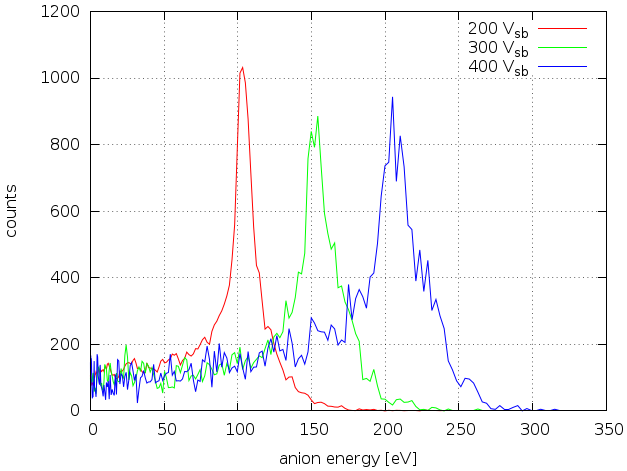
\includegraphics[width=0.8\textwidth]{figures/SFB/ni_cut.png}
            \caption[Negative ion EDF at the anode from 2D]{%
                Negative ion energy distribution at the anode %
                at \SI{4}{\pascal} and 800$V\ix{pp}$ with different %
                self-bias voltages.}
            \label{fig:dist_cut}
        \end{figure}

%%%%%%%%%%%%%%%%%%%%%%%%%%%%%%
%%%%%%% ONEDIMENSIONAL RESULTS
%		\newpage
%        \begin{figure}[!h]
%            \centering
%            \includegraphics[height=0.4\textheight]%
%                {figures/results/2D/ONED/1D_44420_672_potential.png}
%            \caption{%
%                Phase resolved potential of a one-dimensional simulation %
%                at \SI{5}{Pa} and \SI{400}{V}.}
%            \label{fig:2D:onedpotprs}
%        \end{figure}
%        \begin{figure}[!h]
%            \centering
%            \includegraphics[height=0.4\textheight]%
%                {figures/results/2D/ONED/1D_44420_672_dens.png}
%            \caption{%
%                One-dimensional simulation results of %
%                particle densities at \SI{5}{Pa} and \SI{400}{V}.}
%            \label{fig:2D:oneddens}
%        \end{figure}
%        \begin{figure}[!h]
%            \centering
%            \includegraphics[height=0.3\textheight]%
%                {figures/results/2D/ONED/1D_44420_672_prsdens.png}
%            \caption{%
%                One-dimensional simulation results of phase-resolved %
%                densities in front of the driven electrode at %
%                \SI{5}{Pa} and \SI{400}{V}.}
%            \label{fig:2D:twoddensprs}
%        \end{figure}
%        \newpage
%%%%%%%%%%%%%%%%%%%%%%%%%%%%%%%
%%%%%%%% TWODIMENSIONAL RESULTS      
%        \begin{figure}[!h]
%            \centering
%            \includegraphics[height=0.3\textheight]%
%                {figures/results/2D/43748/45365prs_pot.png}
%            \caption{%
%                Two-dimensional simulation results of phase-resolved %
%                potential at the axial centre of the discharge t %
%                \SI{5}{Pa} and \SI{400}{V}.}
%            \label{fig:2D:twodpot}
%        \end{figure}
%        \begin{figure}[!h]
%            \centering
%            \includegraphics[height=0.3\textheight]%
%                {figures/results/2D/43748/45365_dens.png}
%            \caption{%
%                Two-dimensional simulation results of phase-resolved %
%                densities at the axial centre of the discharge in at %
%                \SI{5}{Pa} and \SI{400}{V}.}
%            \label{fig:2D:twoddensright}
%        \end{figure}
%        \begin{figure}[!h]
%            \centering
%            \includegraphics[height=0.3\textheight]%
%                {figures/results/2D/43748/45365prs_dens_left.png}
%            \caption{%
%                Two-dimensional simulation results of phase-resolved %
%                densities at the axial centre of the discharge in %
%                front of the driven electrode at %
%                \SI{5}{Pa} and \SI{400}{V}.}
%            \label{fig:2D:twoddensleft}
%        \end{figure}
%        \newpage
%%%%%%%%%%%%%%%%%
%%%%%%%%%%%%%%%%%